In order to apply an RBAC security policy to the EMS system, we need to define the required components of RBAC models (i.e. $RBAC_0$, $RBAC_1$ and $RBAC_2$).  For $RBAC_0$, it is essential to specify the sets of USERS, ROLES, and PERMISSIONS.

\subsection{$RBAC_0$- Basic Model}
Since the system has three main types of users (i.e. staff, students and students' guardains), each user represents an element in the USER set (U).  Regarding ROLES (R), there are six basic roles, which describe the main functionality for users in the Electronic Marking System.  These roles would be stored into the ROLES entity of the database.  Therefore, contents of this entity can be defined as follows:

\begin{align*}
ROLES = \{admin, student, teacher, headteacher, \\headmaster, student\_guardian\}
\end{align*}


Permissions (P) are pairs of (operations, objects) in which users are allowed to perform.  For example, a student wants to store a report $(operation)$ into SUBMISSION table $(object)$ in order for the report to be considered “submitted”.  This process means that the student is permitted to add a submission.  The EMS system allows each type of users to perform only specific permissions. 

%\begin{figure}[bht]
%\centering
%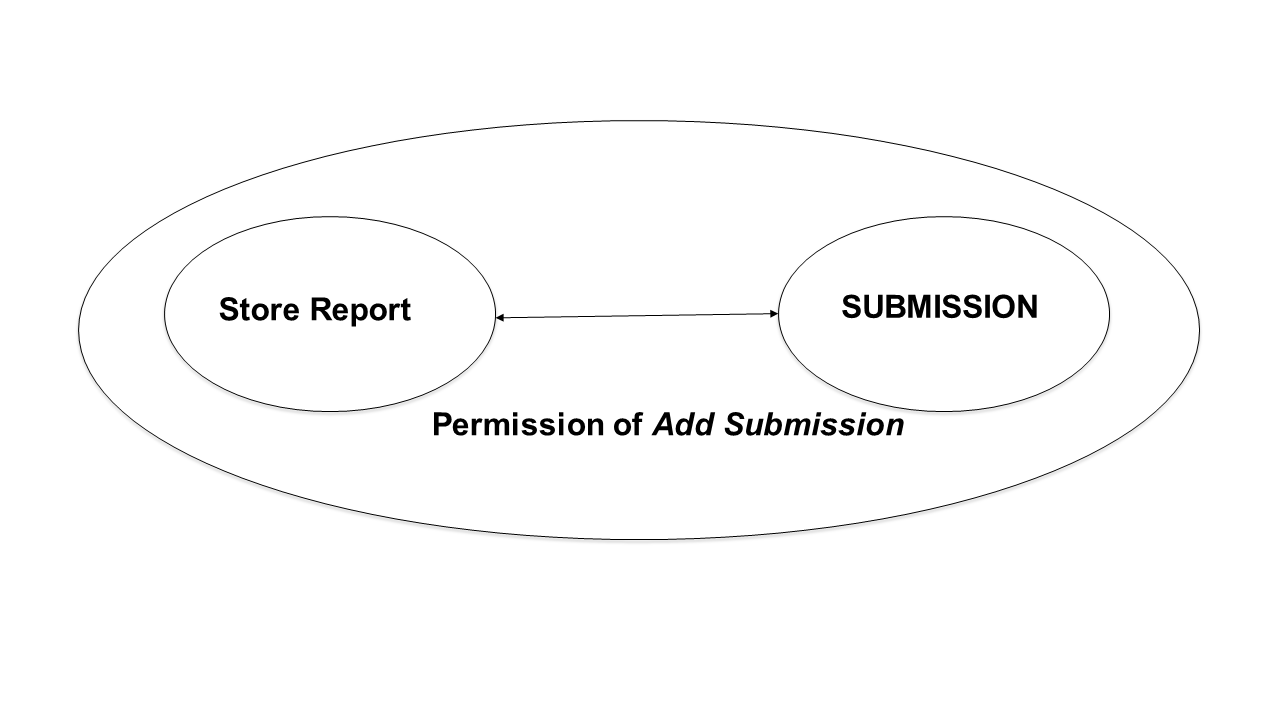
\includegraphics[scale=0.26]{addsubmission.png}
%\caption{"Add Submission" permission for students.}
%\label{fig:permstud}
%\end{figure}

\subsection{User Assignment (UA) and Permission Assignment (PA)}
User Assignment (UA) is a many-to-many relationship between the system users U and the roles R.  For example, students take the role $student$, while teachers are assigned to role $teacher$.  In some cases, it is possible to assign a user to two different roles if a given situation requires that.  For instance, in case of absence of a headmaster, any teacher can be authorized to perform the headmaster permissions, and that would be done through giving the role $headmaster$ to the teacher, in addition to his/her own role.

Permission Assignment (PA) is also a many-to-many relationships in which roles are mapped into permissions (functions).  There are specific functions for each role, where can only be performed by user(s) who is/are assigned to those roles.  Figure 6 shows the $admin$ role and permissions assigned to it.

\begin{figure}[bht]
\centering
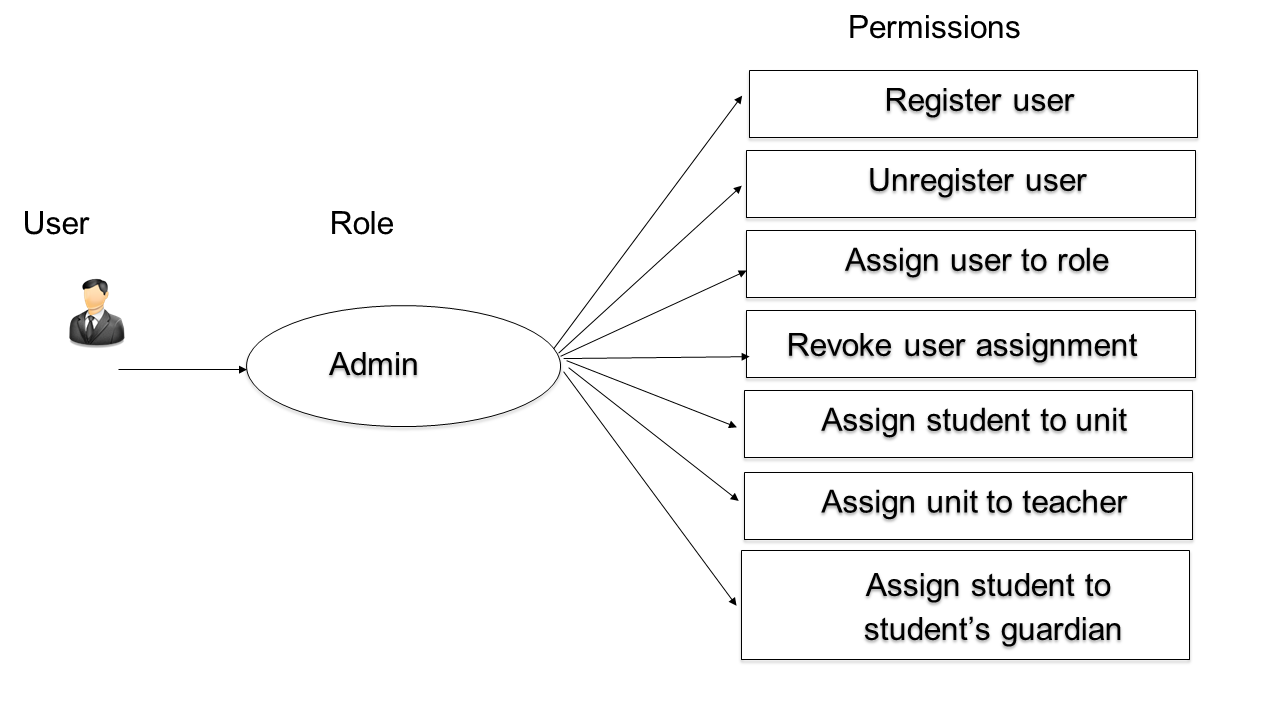
\includegraphics[scale=0.26]{addAdmin.png}
\caption{"Admin" role in the EMS System.}
\label{fig:permstud}
\end{figure}


\subsection{$RBAC_1$- Role Hierarchy (RH)}

In the EMS system, there is only one instance of role hierarchy.  Head teachers are, in fact, teachers, although they have special tasks for organizing and monitoring roles assigned to teachers, such as reviewing records.  When a head teacher is assigned to role $headteacher$, this means that the head teacher is allowed to perform functions of the $headteacher$ role, and inherit permissions from the role $teacher$.

\subsection{$RBAC_2$- Constraints}

For the EMS system, there are two types of constraints that can be defined: cardinality constraints and mutual exclusiveness of roles.  Usually, cardinality constraints represent the number of users who should be assigned to a particular role.  In our system, it doesn't matter how many students to be assigned to $student$ role, or how many teachers to be mapped into $teacher$ role, as that depends on the number of students and teachers inside a certain school.  However, there must be only one user who should take the role $headmaster$.  Thus, the cardinality constraint for that role  is expressed as:

\begin{flalign*}
UA \subseteq U \times R\ \text{where}\ \\ 
\mathbf{card}(U (school manager)) \times \mathbf{card}(R(headmaster)) = 1
\end{flalign*}


Mutual exclusiveness of roles (Separation of Duties) define the conflicted sets of roles, which must not be related to the same user/s.  For example, if there are two roles $R1$ and $R2$ belonging to two conflicted sets of roles $S1$ and $S2$, respectively, then: If a user $U$ has been assigned to a role in $S1$, this implies that $U$ is not assigned to any role in $S2$, and vice versa.  

In the EMS system, there are two conflicted classes (sets) of roles:

\begin{flalign*}
sod1 &= \{teacher, headteacher, headmaster\}, and \\
sod2 &= \{student, student\_guardian\}
\end{flalign*} \\
